\section{OpenMLE-Gym: Building Scalable Verifiable Environments}
\label{sec:framework}
\label{sec:task-curation-data-construction}

\begin{takeaway}
\begin{itemize}[leftmargin=*,itemsep=1pt,topsep=2pt,partopsep=0pt,parsep=0pt]
\item \textbf{MLE requires a compute-backed, verifiable gym.} LLM agents can be improved through interaction with executable, data-grounded environments. For MLE, the environment must host large, resource-intensive tasks, execute candidate programs under controlled budgets, and apply task-specific evaluators to return reproducible diagnostics and rewards. \openmlegym{} provides this substrate for post-training, search, and evaluation toward recursive self-improvement.
\item \textbf{The gym scales through automated task construction.} Our construction and quality-control pipeline turns curated anchors, Kaggle datasets, and Kaggle competitions into 5,758 quality-gated executable environments spanning eight modalities and six core task types, with executability validation and semantic quality gating.
\end{itemize}
\end{takeaway}

AI-for-AI requires agents to build and improve AI systems through executable experimentation, making machine learning engineering (MLE) a concrete testbed for this loop. Such agents need large-scale, diverse, high-quality task packages spanning data inspection, preparation, modeling, prediction, and evaluation. Yet these resources remain scarce: existing benchmarks are limited in openness, executable diversity, or coverage, while heterogeneous files, formats, and evaluation protocols make them difficult to scale.

Static task collections alone do not support post-training or search. Agent-generated programs must execute under controlled resources and produce reliable, informative feedback that guides subsequent actions. Gym-style environments make this interaction contract explicit by coupling tasks with actions, transitions, observations, rewards, and stopping conditions~\citep{brockman2016openai,xi2024agentgym,nathani2025mlgym,qiang2025mledojo}. OpenMLE-Gym therefore unifies scalable executable tasks with standardized packages, isolated execution, structured diagnostics, and task-specific evaluation for post-training, test-time search, and AI-for-AI.

\subsection{Environment Contract}
\label{sec:gym-environment-contract}
Each OpenMLE-Gym task is an environment instance defined by five elements. The task/state consists of the task specification, public data, hidden evaluator, resource budget, and current workspace state. The action is an agent-submitted MLE program together with its execution requirements. The transition is sandbox execution: the environment materializes the workspace, runs the program against public data, and invokes the evaluator when a valid submission is produced. The observation is a structured record containing execution status, task score, logs, error types, generated artifacts, and runtime metadata. The reward is the verifiable task-specific score returned by the evaluator.
Task completion, controller stopping criteria, and time or compute budgets determine whether an interaction terminates or is truncated.


\begin{figure}[t]
  \centering
  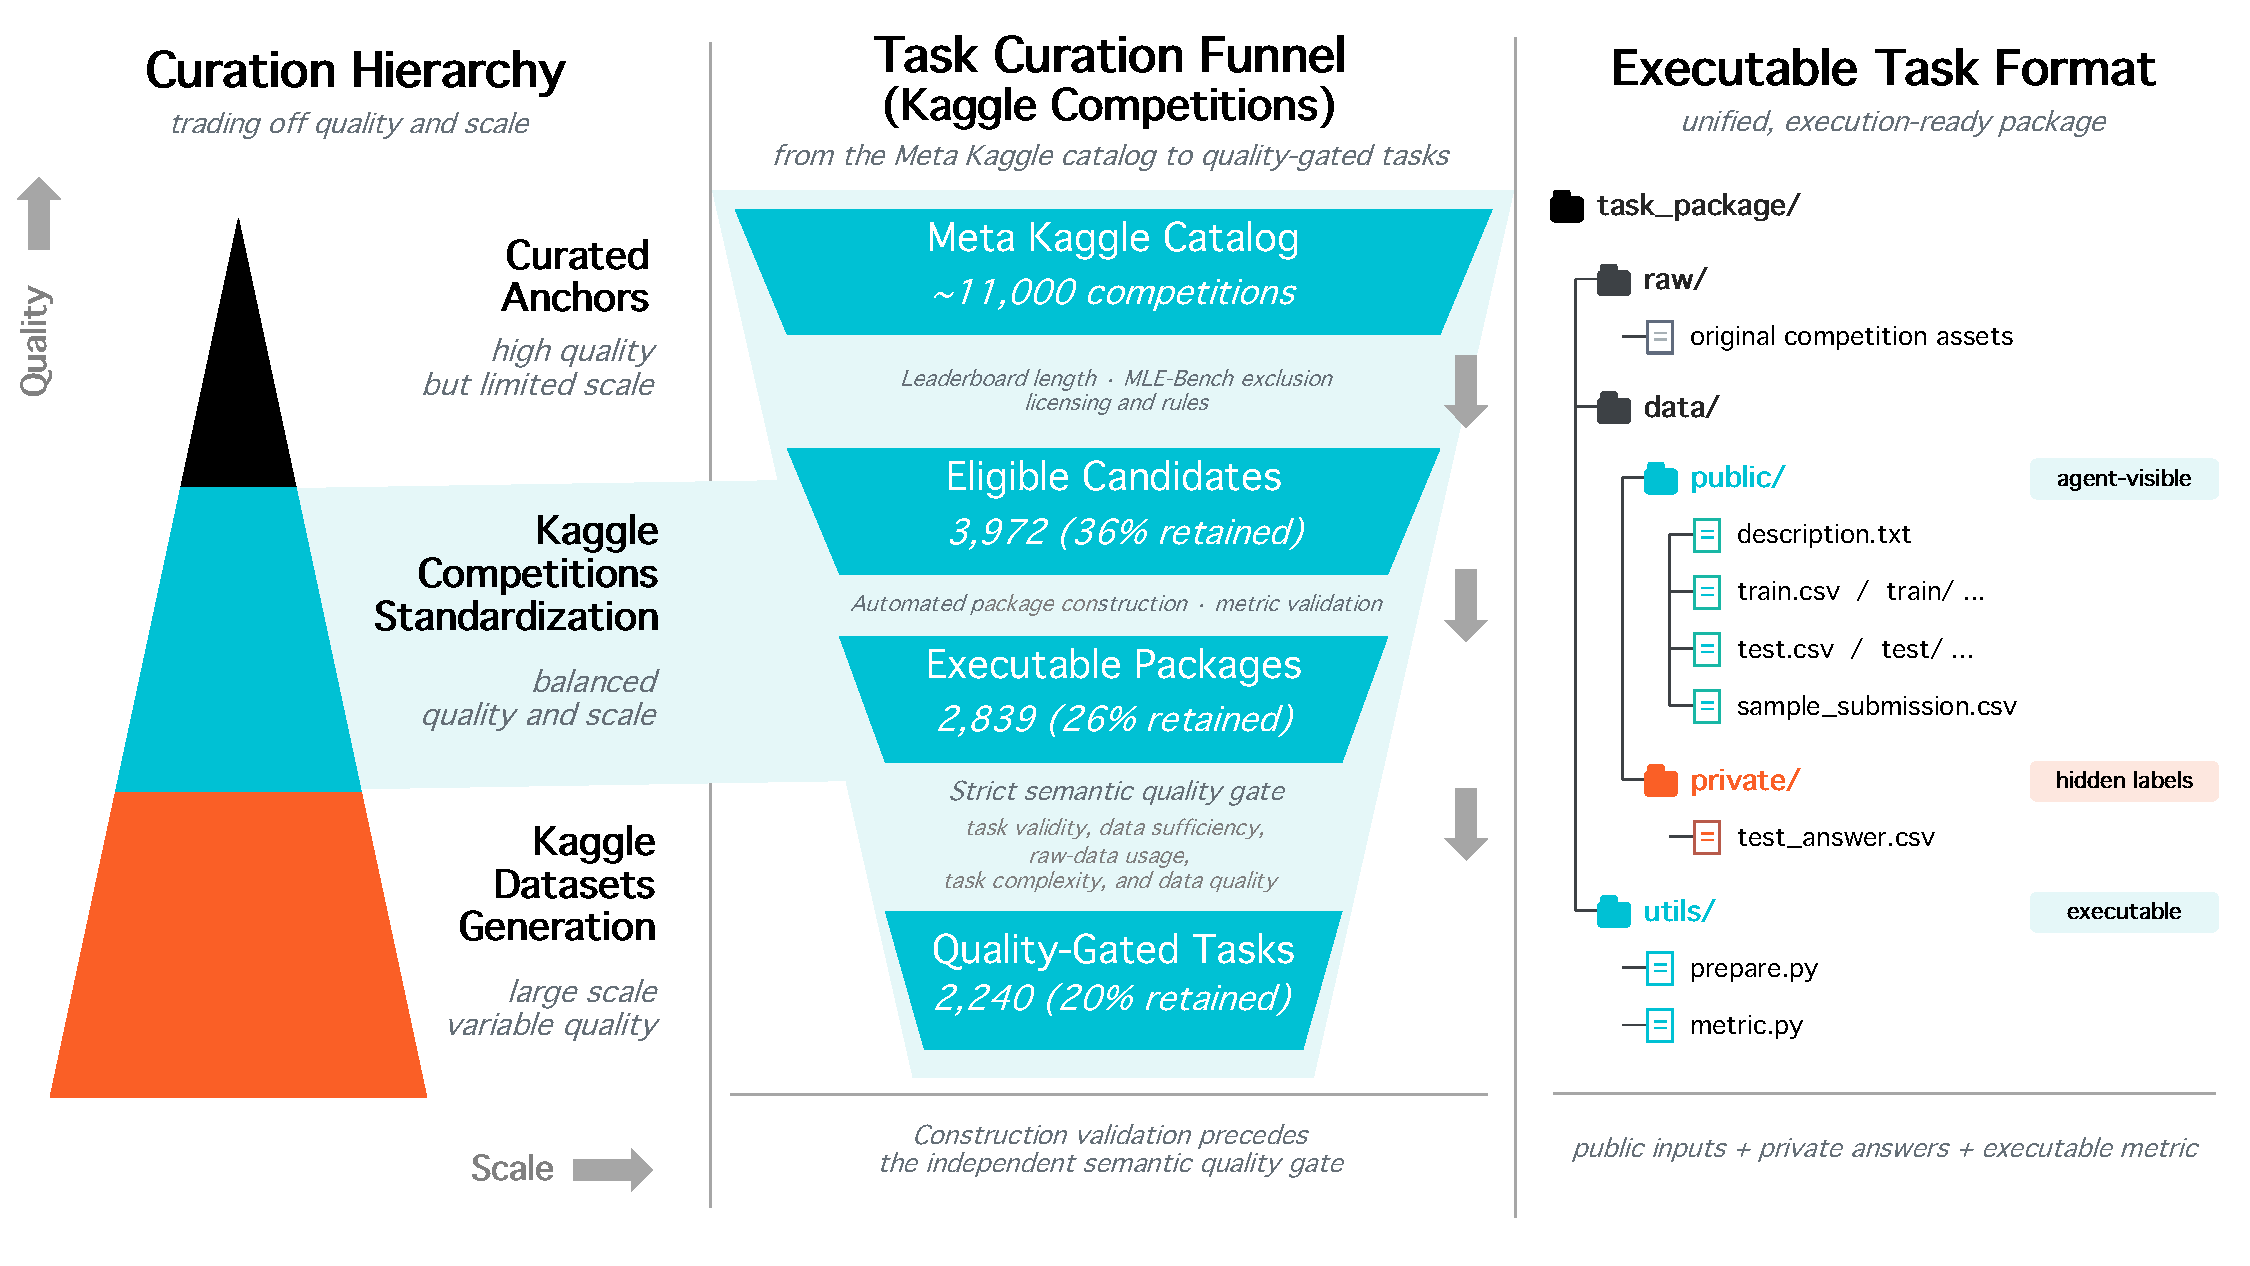
\includegraphics[page=1,width=\linewidth]{figures/task-curation.pdf}
  \caption{OpenMLE-Gym task curation and executable format. \textbf{Left:} source hierarchy. \textbf{Middle:} Kaggle Competition filtering from the Meta Kaggle catalog to quality-gated packages. \textbf{Right:} public task inputs, private answers, and executable utilities.}
  \label{fig:task-curation-summary}
\end{figure}

\subsection{Scalable Task Construction}
\textbf{OpenMLE-Gym} is our unified executable task suite, constructed from three source-specific paths that occupy complementary positions in the quality--scale trade-off (Figure~\ref{fig:task-curation-summary}, left). \textbf{Curated Anchors} provide the highest-confidence task designs because they are manually selected from existing papers and benchmarks, but their dependence on prior expert curation limits scale. We download their original assets and process them directly into executable packages. \textbf{Kaggle Datasets} substantially broaden task and data coverage, although automatically induced objectives can have more variable quality. We utilize and extend the existing MLE-Smith dataset-to-task pipeline~\citep{qiang2025mlesmith}, then apply package-level quality control. \textbf{Kaggle Competitions} offer a middle ground: human-authored problem specifications, evaluation metrics, and submission protocols provide stronger task grounding, while prior participant engagement and leaderboard records offer additional external evidence that tasks support meaningful, comparable evaluation. Meanwhile, the Meta Kaggle catalog supports collection at scale. We build our own crawling and competition-construction pipeline, with MLE-Bench-overlapping competitions excluded to preserve evaluation integrity.

Following the principles of MLE-Dojo~\citep{qiang2025mledojo}, we map all three sources into a shared executable task package. Original assets remain under \texttt{raw/}. Agent-visible descriptions, training data, test inputs, and sample submissions are placed under \texttt{data/public/}, while hidden answers are isolated under \texttt{data/private/}. A task-specific \texttt{metric.py} validates prediction files and returns scalar execution feedback. This contract gives heterogeneous tasks the same agent-facing interaction surface while preserving their original semantics.

For the competition-derived branch, our automated framework converts a Kaggle competition slug into a standardized executable package. It downloads and inventories the competition files, then combines local evidence---including schemas, data types, dimensions, and sampled rows---with Meta Kaggle records describing the problem, evaluation criterion, and submission protocol. From this grounded context, the framework constructs the task description and generates \texttt{prepare.py} to deterministically split labeled data, isolate public inputs from private answers, and produce a schema-compatible sample submission. It then generates \texttt{metric.py} and validates the complete package by executing the preparation code and scoring the sample submission. Failures and assertion errors are returned as feedback for bounded retries; packages that remain unbuildable or fail to produce a valid scalar metric are removed before semantic quality filtering. A detailed stage-by-stage view is provided in Appendix~\ref{app:data-construction} (Figure~\ref{fig:competition-task-construction}).

\subsection{Task Quality Filtering}
To ensure the quality of constructed task packages, we propose an LLM-based quality filter. For each task package, the filter jointly inspects the task description, raw files, processing script, processed outputs, representative data samples, etc. It returns structured judgments along five dimensions: task validity, data sufficiency, raw-data usage, task complexity, and data quality. Together, these criteria identify degenerate targets solvable by trivial rules, inadequate training or evaluation signal, superficial use of source assets, mismatched difficulty, data leakage, annotation errors, and malformed processing. For example, the competition branch applies this final semantic gate only after leaderboard-length screening, MLE-Bench overlap removal, licensing and competition-rule screening and executable package and metric validation (Figure~\ref{fig:task-curation-summary}, middle). We retain only metric-valid tasks receiving the strict \texttt{recommended} decision, thereby separating semantic quality assessment from the executability check performed during construction.

\begin{figure*}[!t]
  \centering
  \includegraphics[page=2,width=\textwidth]{figures/task-curation.pdf}
  \caption{Scale and composition of OpenMLE-Gym. \textbf{Left:} comparison with executable task-package resources and source breakdown of 5,758 tasks. \textbf{Right:} normalized modality, task-type, and non-raw package-size distributions.}
  \label{fig:task-scale-distribution}
\end{figure*}

\subsection{Sandbox Execution at Scale}
\label{sec:gym-sandbox-execution}
The contract is realized at scale by a shared sandbox execution backend. A centralized scheduler receives API requests, records each job, tracks worker availability, and dispatches requests to CPU/GPU Docker workers according to resource requirements. Each worker materializes an isolated task workspace, mounts the task data and evaluator, executes the candidate program, and writes logs, submissions, outputs, and artifacts back to shared storage. This separation of control, execution, and storage supports reproducible scoring and scalable parallel execution across long-running MLE jobs.

The backend returns six feedback modes: successful completion, runtime error, missing code, missing submission, scoring failure, and timeout. Each record preserves the triggering condition together with status, score when available, logs, error type, runtime metadata, and workspace artifacts, allowing the agent to distinguish invalid execution from weak task performance. Detailed architecture and representative feedback cases are provided in Appendix~\ref{app:sandbox}.



\subsection{Composition and Statistics}
OpenMLE-Gym contains 5,758 executable tasks\footnote{Owing to source-data licensing and copyright constraints, we release full task-package data for 1,415 tasks. For the remaining 4,343 tasks, we release the corresponding \texttt{prepare.py} and \texttt{metric.py} scripts without redistributing the source data.}: 156 manually selected Curated Anchors, 3,362 Kaggle Dataset tasks generated from the official MLE-Smith table and quality-controlled at the package level, and 2,240 tasks retained from our Kaggle Competition pipeline (Figure~\ref{fig:task-scale-distribution}, left). Across the three sources, the pool covers tabular, text, time-series, image, and other data modalities, with classification and regression complemented by more engineering-intensive task types. After canonicalizing modality and task-type labels, 11\% of tasks are multimodal and classification and regression together account for 87\% (Figure~\ref{fig:task-scale-distribution}, right). Additional construction details are provided in Appendix~\ref{app:data-construction}.

\section{OpenMLE-ERL: Reinforcing Reusable Evolutionary Operators}

\begin{takeaway}
    \begin{itemize}[leftmargin=*,itemsep=1pt,topsep=2pt,partopsep=0pt,parsep=0pt]
    \item \textbf{RSI training should improve the best solution a model can find within a fixed budget.} 
    Execution-grounded SFT increases strong solutions and useful revisions under repeated sampling; RL uses adaptive score bounds and entropic advantages to reward candidate quality rather than validity alone.
    \item \textbf{Verification cost must shape collection and training.} Budget-adaptive SFT stops at an accepted-example quota or execution limit, preserving budget for sparse-success tasks; asynchronous RL admits completed generation-and-execution groups immediately instead of waiting for the slowest job.
    \item \textbf{Evolutionary search depends on learning revisions, not only fresh drafts.} 
    We train \textsc{Draft}, \textsc{Improve}, \textsc{Debug}, and \textsc{Crossover} from trajectory transitions; stateful RL selects parents using reward, child-reward variance, and visit-based cooling.
    \end{itemize}
\end{takeaway}

\textbf{Motivation.}
Evolutionary AutoResearch is judged by the best executable program found within a finite search budget. A controller may invoke \textsc{Draft}, \textsc{Debug}, \textsc{Improve}, and \textsc{Crossover} hundreds or thousands of times, so the model must learn more than one-shot solution generation: it must repeatedly repair, refine, and recombine programs as the search unfolds. Post-training should therefore expand the set of strong programs reachable through repeated sampling while improving the individual transformations that the inference harness composes.


SFT and RL play complementary roles in meeting this objective. Execution-grounded SFT distills complete solutions and successful local revisions from stronger teachers, giving the model a broader set of executable behaviors before online learning begins. RL then moves probability toward the better candidates within that broadened distribution. This division is motivated by prior analyses of RLVR: RL can raise Pass@1 by reinforcing already-rewarded solutions yet provide limited gains at large $K$, whereas teacher distillation can introduce behaviors absent from the base model's sampled support~\citep{yue2025doesrl}.

Executable evolutionary training also differs from short-horizon RLVR on mathematics and code generation~\citep{shao2024deepseekmath}. Many programs fail to produce a usable reward, while successful programs receive continuous task scores drawn from different metrics and ranges. Feedback arrives only after sandbox runs that may last minutes or hours, and every non-\textsc{Draft} action depends on the parent program selected for expansion. OpenMLE-ERL addresses these constraints across both stages: SFT collection uses execution results and per-task budgets to select useful supervision, while RL preserves score differences among strong candidates, removes synchronization stalls, and trains each operator on informative program states.

\begin{figure}[!htbp]
  \centering
  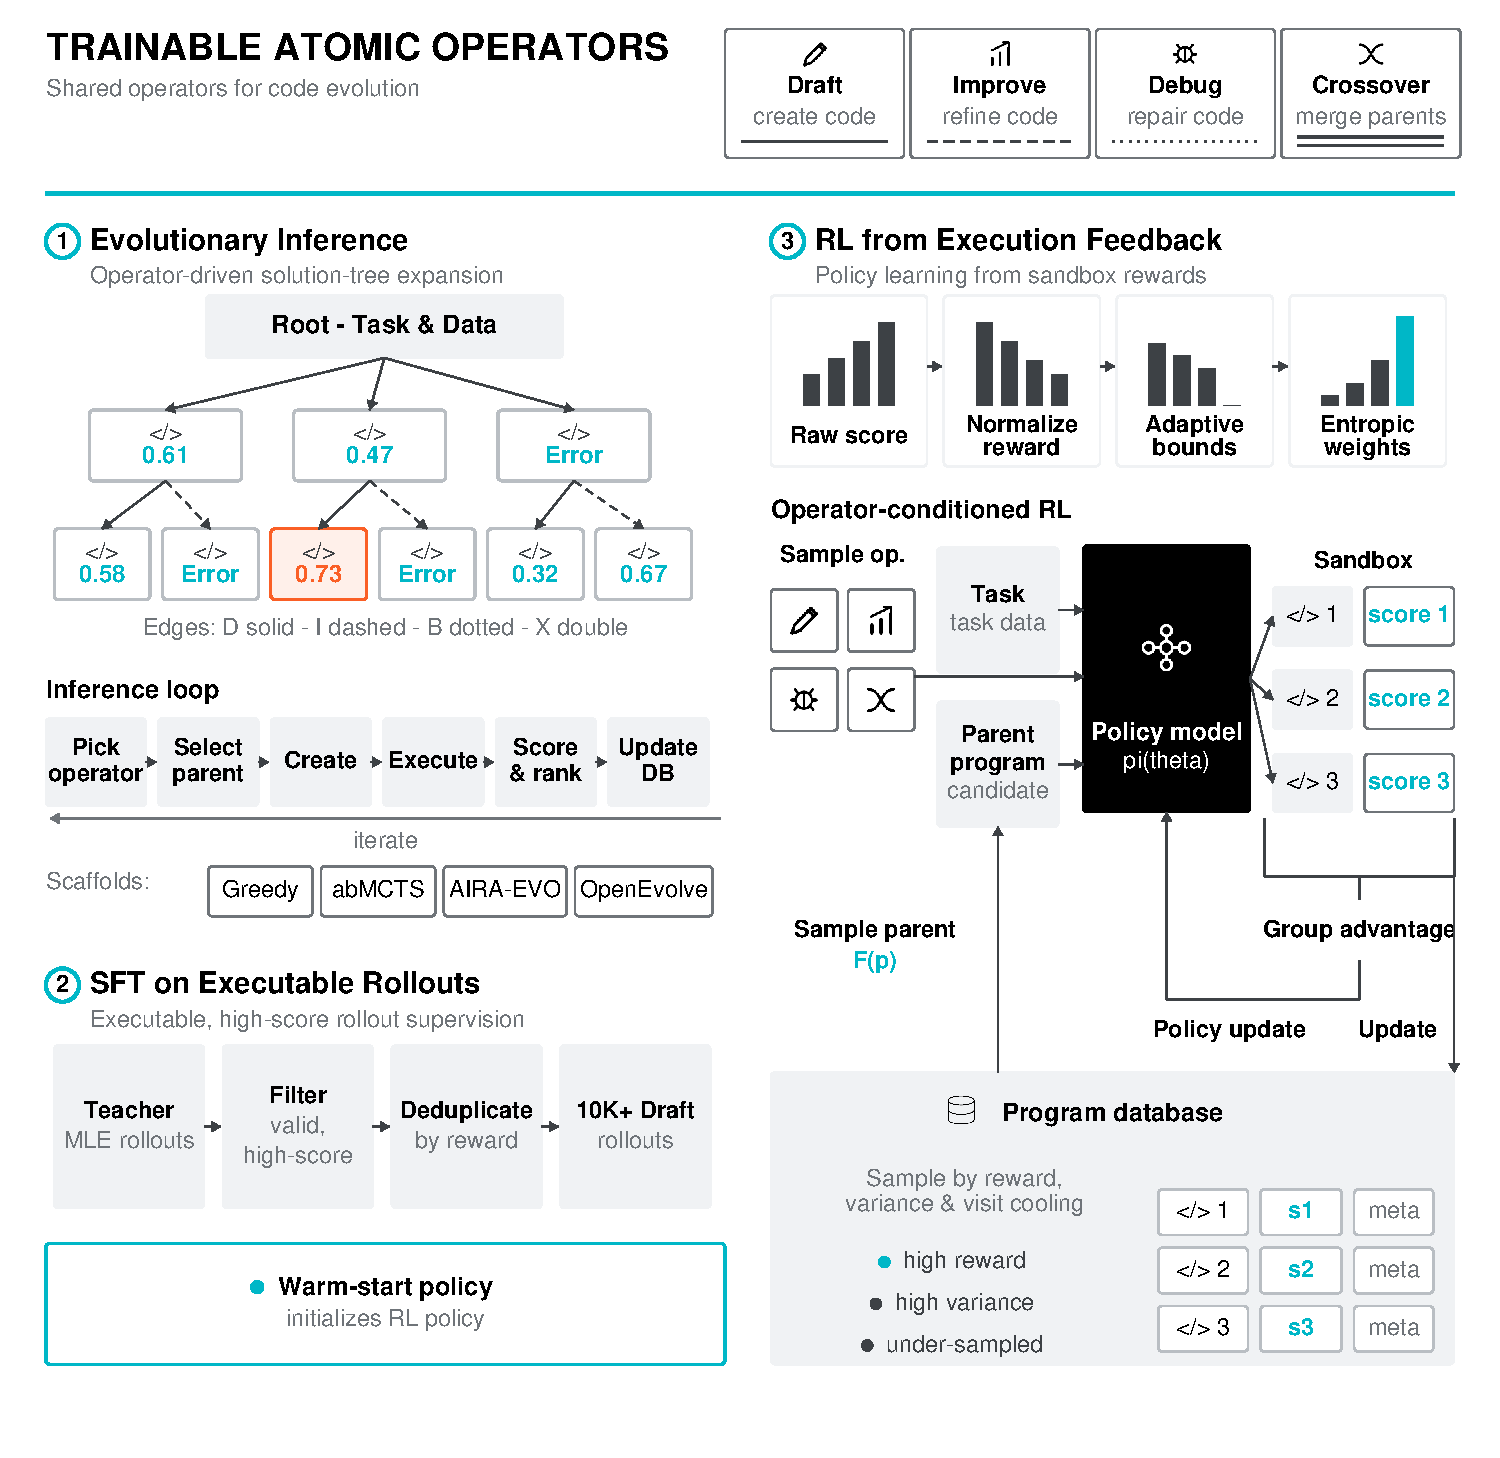
\includegraphics[width=\textwidth]{figures/frontis-method-figure.pdf}
  \caption{Overview of the OpenMLE training and inference workflow. Trainable atomic operators are used by evolutionary inference, warm-started through executable SFT rollouts, and further optimized with online RL from execution feedback.}
  \label{fig:openmle-framework}
\end{figure}


\subsection{Trainable Atomic Operators for Evolutionary Inference}
\label{sec:atomic-operators}

A central design principle of OpenMLE is to separate the local skills learned by the model from the search algorithm used at inference time. Rather than training full trajectories, OpenMLE trains a compact set of reusable program-transformation operators over executable candidates. This avoids sparse controller-specific supervision and lets the same learned operators be composed by different evolutionary search procedures under a shared sandbox protocol.

We instantiate the atomic operators as \textsc{Draft}, \textsc{Improve}, \textsc{Debug}, and \textsc{Crossover}. This operator vocabulary follows AIRA-style executable MLE search and AIDE-style code-space exploration~\citep{toledo2025airesearchagents,hambardzumyan2026aira_2,jiang2025aide}, but OpenMLE adapts it as explicit SFT and RL targets for open-model post-training.
Detailed operator definitions, prompt templates, and controller-specific search details are provided in the appendix.

\subsection{Execution-Grounded Supervised Warm Start}
\label{sec:supervised-warm-start}




\textbf{Execution-grounded, budget-adaptive collection.}
For each task, we execute sampled programs in the sandbox and retain examples according to their validity and task-specific scores. Collection stops when either an accepted-example quota is reached or the task exhausts its execution budget, allowing easy tasks to terminate early while allocating more attempts to tasks with sparse successes. This difficulty-aware rejection strategy directs verification compute toward tasks for which further exploration can still recover useful supervision~\citep{tong2024dartmath}.

\textbf{Parallel and evolutionary sampling paths.}
The \emph{parallel path} independently samples and executes complete \textsc{Draft} solutions, contributing 17,245 full-response examples to the released corpus. The \emph{evolutionary path} applies \textsc{Improve}, \textsc{Debug}, and \textsc{Crossover} over executed programs and retains useful steps from high-quality local trajectory segments, contributing 9,014 trajectory-step examples. Figure~\ref{fig:sft-rl-rollout} illustrates both paths. Overall, the two paths form the 26,259-example SFT corpus released with OpenMLE; detailed corpus statistics are provided in Appendix~\ref{app:sft-warm-start}.

\subsection{Execution-Grounded Reinforcement Learning}
\label{sec:execution-grounded-rl}


\begin{figure}[H]
  \centering
  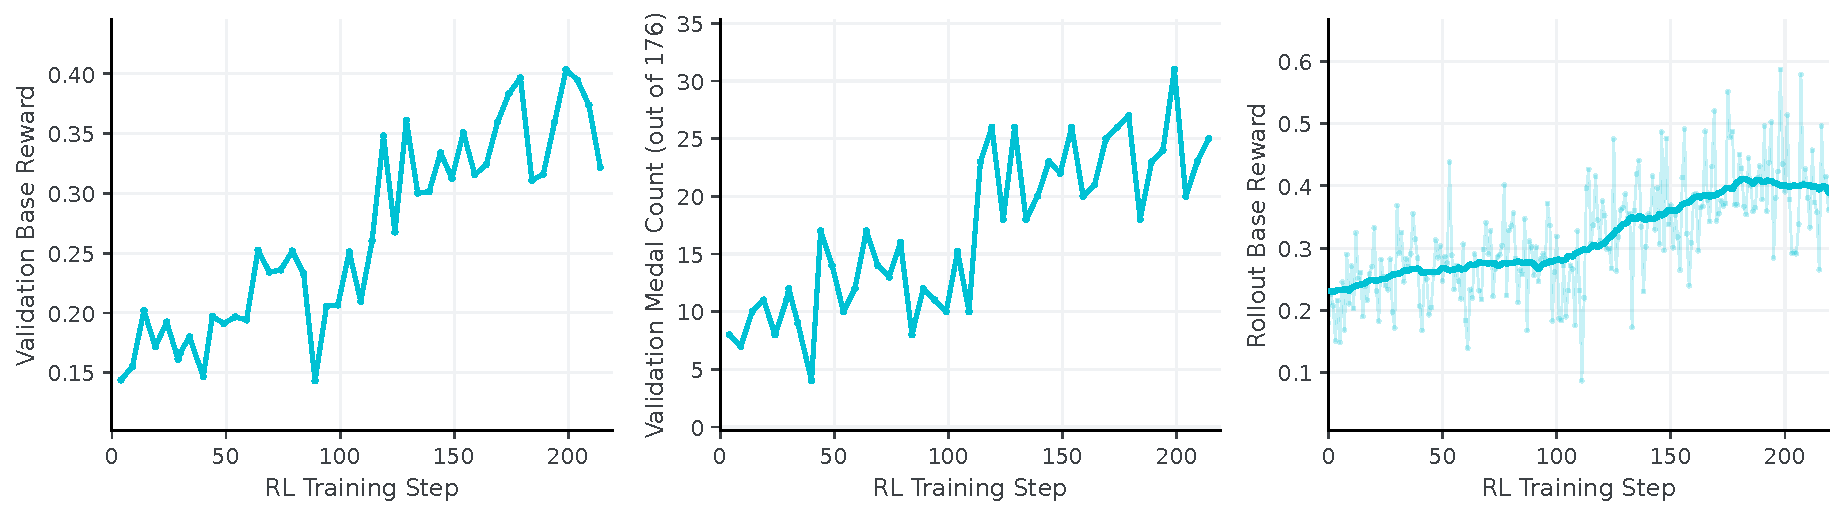
\includegraphics[width=\linewidth]{figures/qwen36_rl_curves.pdf}
  \caption{RL training curves for \thirtyfivebmodel{}.}
  \label{fig:qwen36-rl-curves}
\end{figure}

Building on the supervised warm start, the reinforcement-learning portion of Figure~\ref{fig:sft-rl-rollout} previews how state selection, adaptive reward normalization, and upper-tail weighting act on an evolutionary rollout.

\begin{figure}[H]
  \centering
  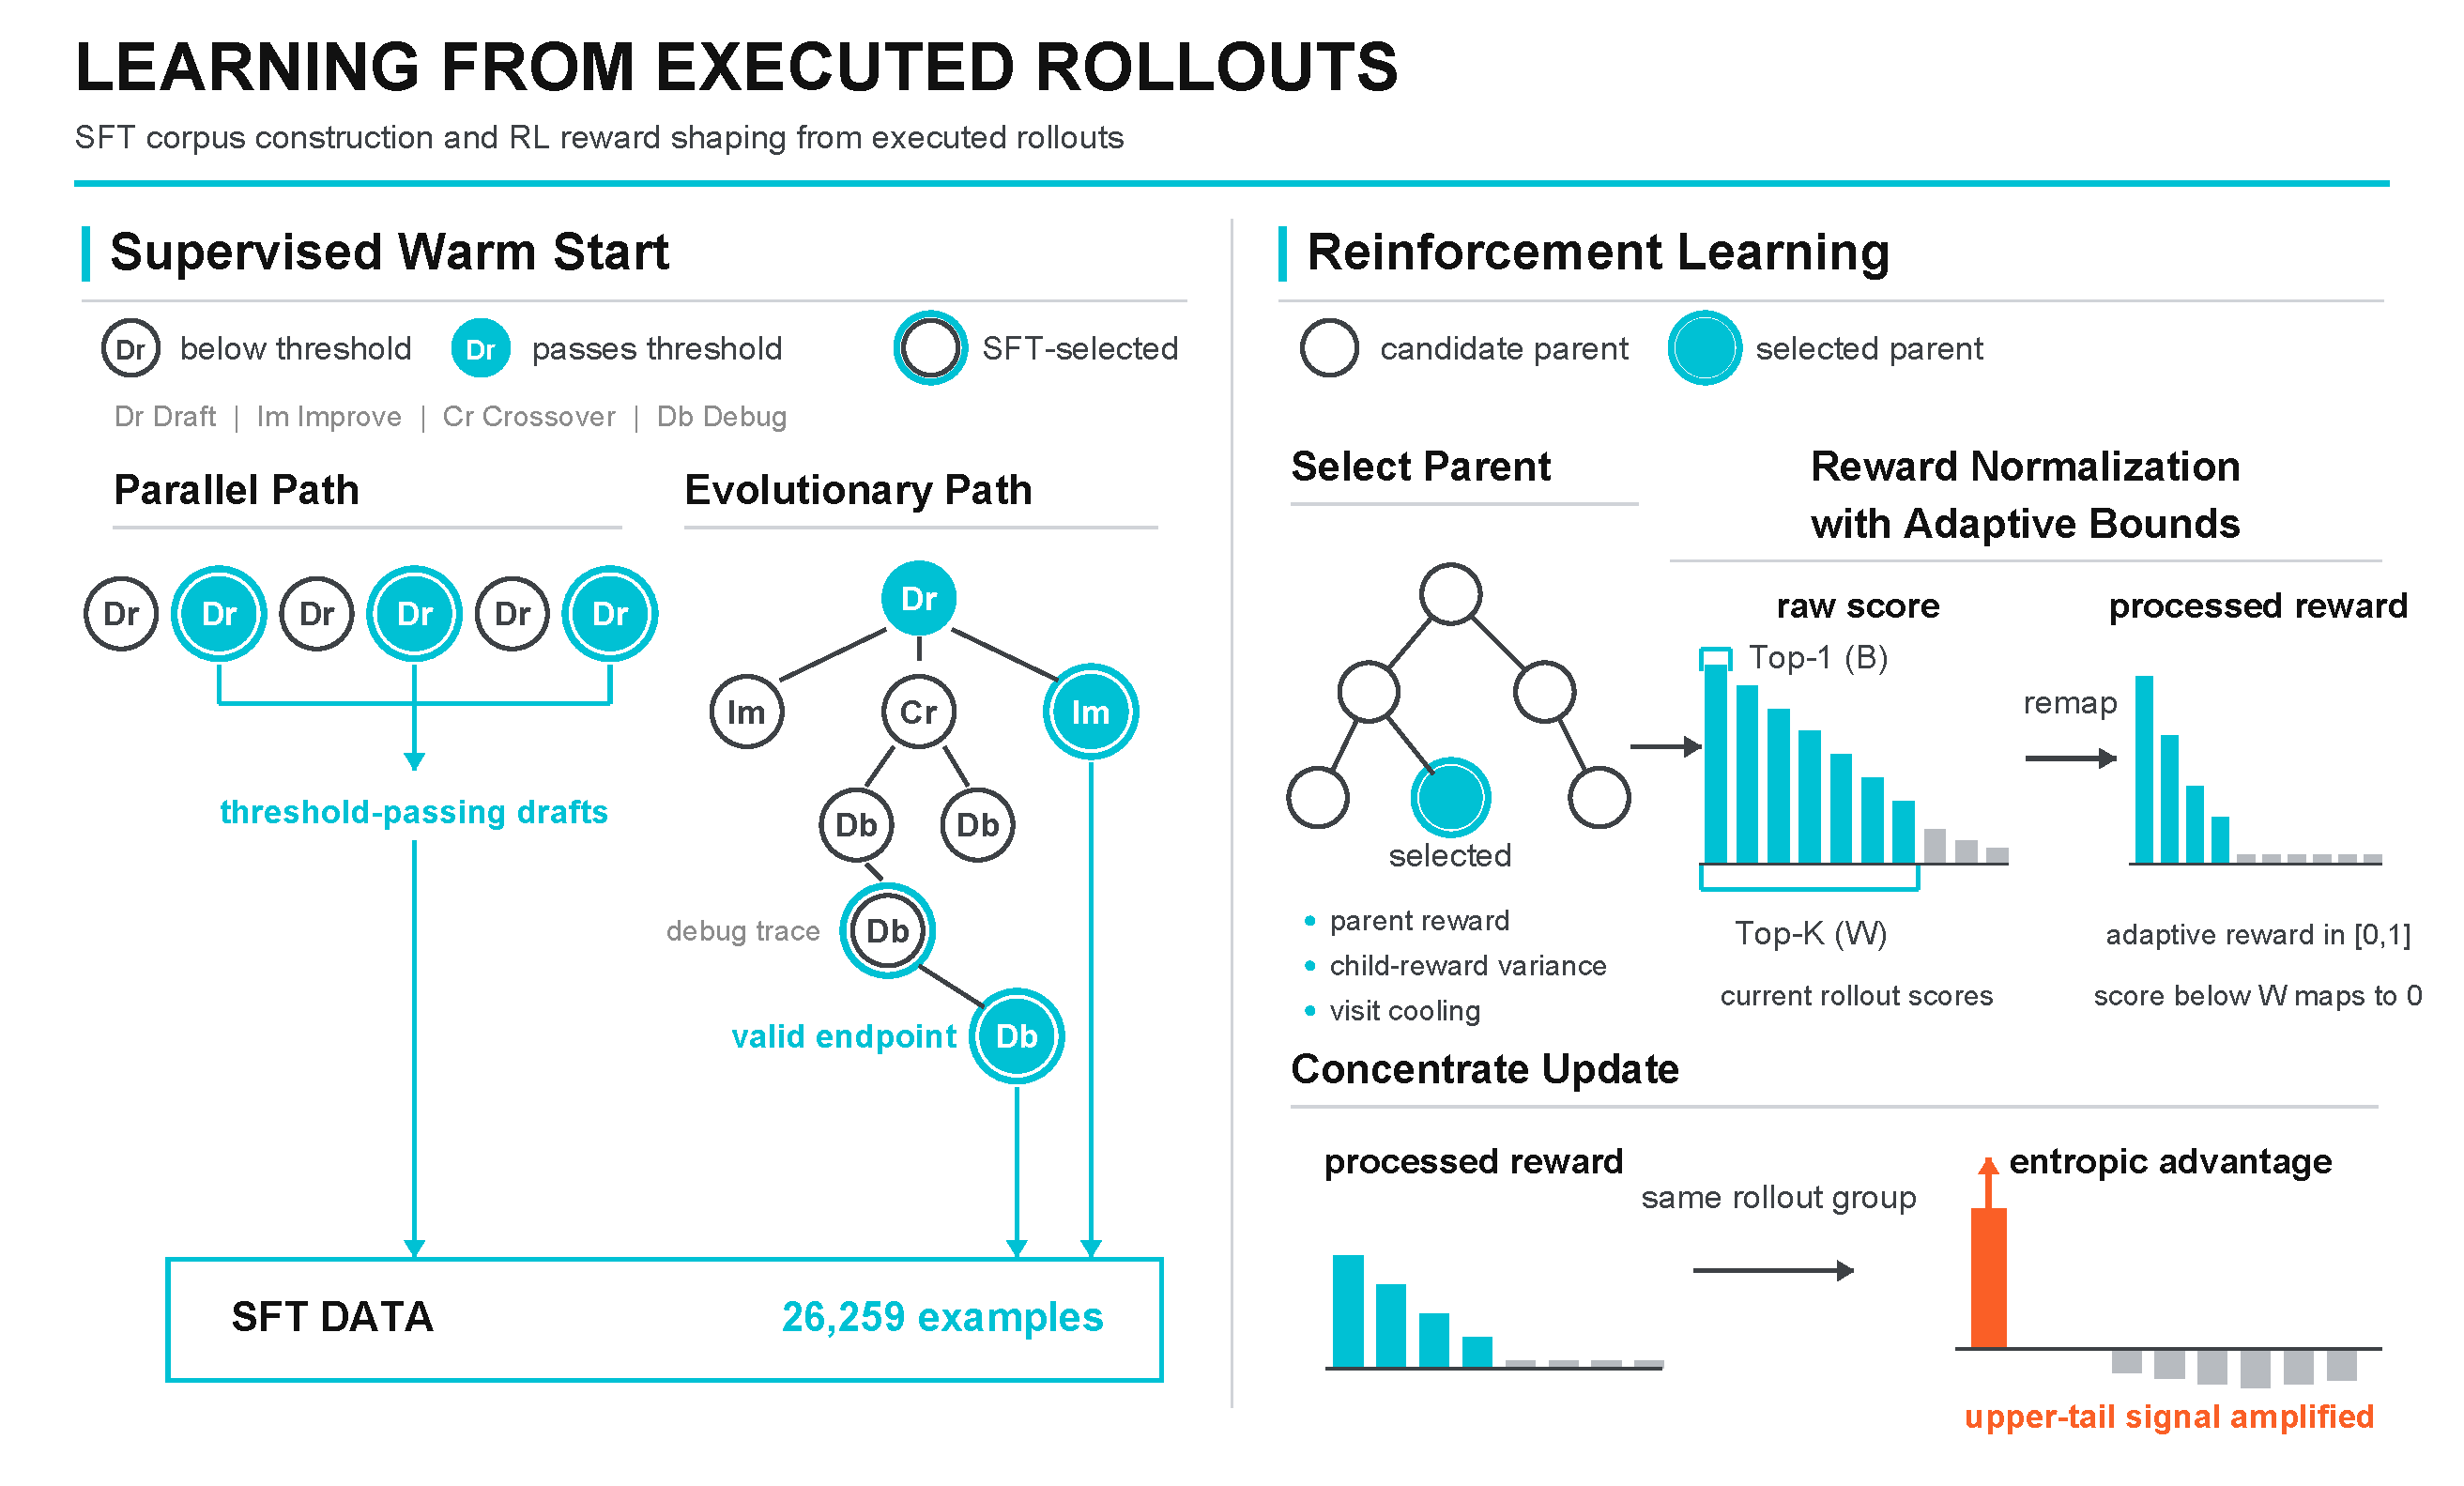
\includegraphics[width=\linewidth]{figures/learning-from-rollouts.pdf}
  \caption{Learning from executed rollouts. The Parallel Path retains threshold-passing \textsc{Draft} solutions. In the Evolutionary Path, a valid endpoint can emerge only after repeated \textsc{Debug} steps; we trace back to the preceding non-debug operator and use an LLM to retain useful steps from that repair trace. The selected examples from both paths form the 26,259-example released SFT corpus under a budget-adaptive stopping rule. For a chosen operator, RL selects a parent using parent reward, child-reward variance, and visit cooling. Top-1/Top-$K$ adaptive bounds map seven nonzero task scores to four nonzero processed rewards in the illustrative rollout group, with scores below the resolved lower bound clipped to zero; entropic advantages then amplify the upper-tail learning signal.}
  \label{fig:sft-rl-rollout}
\end{figure}

\textbf{Making heterogeneous outcomes comparable.}
One task may optimize accuracy and another log loss; even after aligning their directions, raw score ranges remain incomparable. Let $\tilde{s}$ denote a raw score converted to the convention that larger is better. We first define a bounded \emph{base reward} from a fixed pair of task bounds:
\begin{equation}
\label{eq:base-reward}
r_{\mathrm{base}}(\tilde{s}; b_{\mathrm{best}}, b_{\mathrm{worst}}) =
\mathrm{clip}\left(\frac{\tilde{s} - b_{\mathrm{worst}}}{b_{\mathrm{best}} - b_{\mathrm{worst}}}, 0, 1\right)^\alpha,
\qquad \alpha > 0.
\end{equation}
Fixed bounds establish a common interval, but leaderboard or theoretical extrema can be much wider than the score region reached by the current policy. In that case, meaningfully different programs collapse to nearly identical rewards. OpenMLE therefore derives tighter adaptive bounds from each task's historical on-policy score frontier and remaps $\tilde{s}$ to a processed reward $r_{\mathrm{proc}}$. The bounds evolve with the policy, preserving resolution where current candidates actually lie while retaining a stable reward direction. This follows the broader lesson from adaptive verifiable learning environments and evolving-rubric training that the evaluator scale must preserve discriminative on-policy feedback~\citep{zeng2025rlve,shao2025dr}. Appendix~\ref{app:reward-advantage} specifies the bound construction and edge-case handling.

\textbf{Concentrating learning signal on the upper tail.}
After scores become comparable, the remaining question is how strongly each candidate should affect the update. MLE evaluation rewards the quality of the best program found; a barely viable submission should therefore not receive the same positive reward as a top-performing one. OpenMLE uses an entropic advantage that amplifies reward gaps near the top of each rollout group, following the upper-tail principle studied in TTT-Discover~\citep{yuksekgonul2026learning} and related Best-of-$N$/Pass@$k$ objectives~\citep{walder2025passkpolicy,chen2025passk,bagirov2025bestofn,peng2025simko}. Omitting the stabilizing max-centering used in implementation, the transform is
\begin{equation}
\label{eq:adv}
A_i^{\mathrm{ent}}\approx
\frac{\exp(\beta r_{\mathrm{proc},i})}
{\frac{1}{G-1}\sum_{j\ne i}\exp(\beta r_{\mathrm{proc},j})}
-1,
\end{equation}
where $\beta$ controls concentration and is selected under a fixed entropy/KL budget. These advantages replace the usual GRPO-style group-normalized signal in the clipped policy objective. Adaptive bounds first make within-group differences visible; entropic weighting then directs substantially more learning signal to the best candidates rather than uniformly reinforcing all non-failing programs. Figure~\ref{fig:entropic-advantage-effect} shows both the resulting best-candidate emphasis and its observed effect during training. Exact post-processing formulas appear in Appendix~\ref{app:reward-advantage}.

\begin{figure}[!t]
  \centering
  \begin{minipage}[t]{0.425\linewidth}
    \centering
    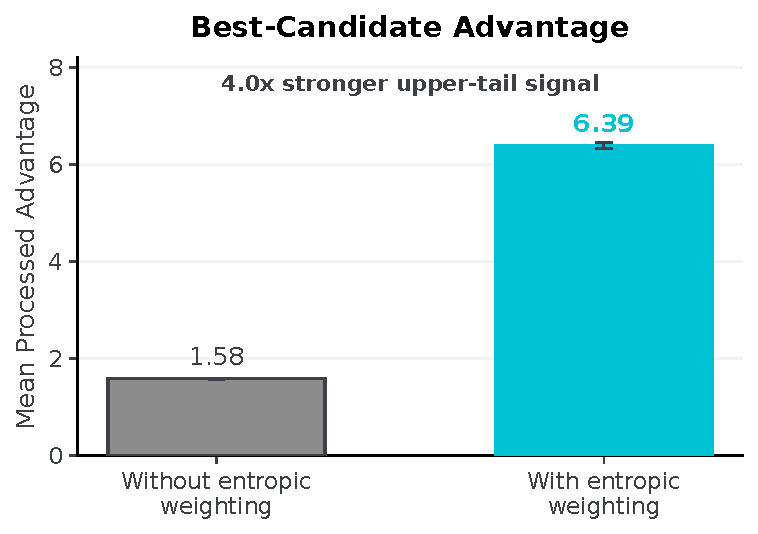
\includegraphics[width=\linewidth]{figures/entropic_advantage_effect.pdf}\\[-0.5ex]
    \small (a) Entropic advantage signal
  \end{minipage}
  \hfill
  \begin{minipage}[t]{0.55\linewidth}
    \centering
    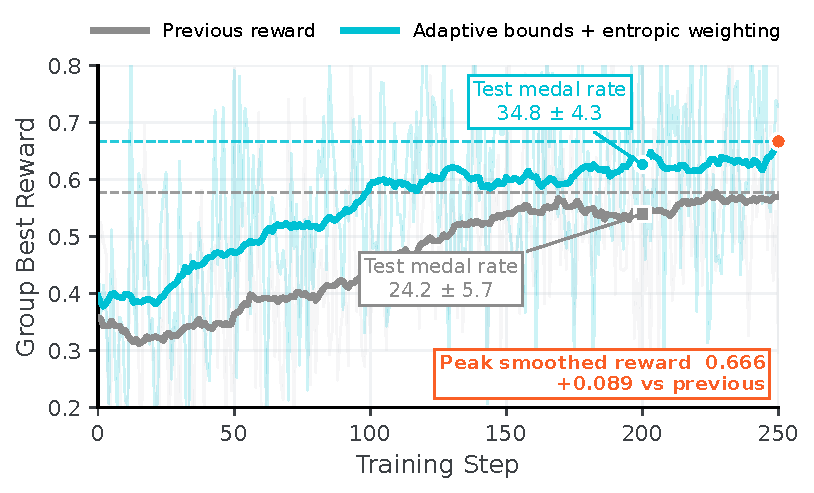
\includegraphics[width=\linewidth]{figures/group_best_reward_comparison.pdf}\\[-0.5ex]
    \small (b) Group Best Reward
  \end{minipage}
  \caption{Effect of upper-tail reward shaping. (a) Entropic weighting increases the processed advantage assigned to the best candidate in a rollout group. (b) Combining entropic weighting with adaptive bounds yields a stronger smoothed Group Best Reward trajectory than the previous reward construction. The two test medal rates in panel (b) use a simpler early-stage harness rather than \openmleevo{}.}
  \label{fig:entropic-advantage-effect}
\end{figure}

\textbf{Removing stragglers with asynchronous rollouts.}
Unlike token-level verification, the dominant latency in MLE RL comes from executing candidate programs, and runtimes vary substantially across tasks and solutions. In a synchronous batch, completed groups remain idle until its slowest sandbox job returns. OpenMLE instead launches generation-and-execution groups independently and lets the trainer consume each completed group from a queue. This decouples policy updates from the longest job in a nominal batch while preserving group-level advantages. Because the realized speedup depends on the task-runtime distribution and worker allocation, we keep the main-text claim qualitative and report the measured timing study in Appendix~\ref{app:async-rollouts}.

\textbf{Selecting informative states for operator learning.}
Evolutionary RL must choose not only a task and an operator, but also the program state on which that operator acts. Uniform parent sampling spends updates on exhausted or uninformative regions; greedy sampling repeatedly trains on the current incumbent and suppresses diversity. After selecting the operator to practice, OpenMLE samples parent programs with a fitness-proportional utility that combines three terms:
\begin{equation}
\label{eq:sample}
F(p) = \mathrm{norm}(R_p) + \mathrm{norm}(\mathrm{Var}_{c \in \mathrm{child}(p)} R_c) + \mathrm{norm}(C_p),
\end{equation}
Here $R_p$ favors strong parent programs, child-reward variance $\mathrm{Var}_{c \in \mathrm{child}(p)} R_c$  identifies regions where operator outcomes remain informative, and $C_p$ is a cooling coefficient that decreases with repeated visits. The first term exploits promising solutions, the second targets states with unresolved learning signal, and the third prevents a single incumbent from monopolizing the rollout budget. This selection rule exposes \textsc{Improve}, \textsc{Debug}, and \textsc{Crossover} to useful yet diverse local contexts; Appendix~\ref{app:evolutionary-fitness} gives the exact implementation.

\section{OpenMLE-Evo: Scaling Experience-driven Long-Horizon Search}
\label{sec:tts-harness}

\begin{takeaway}
\begin{itemize}[leftmargin=*,itemsep=1pt,topsep=2pt,partopsep=0pt,parsep=0pt]
\item \textbf{Test-time scaling becomes test-time learning when search learns from experience.} For AI-for-AI and recursive self-improvement, generating more candidates is not enough: the search process must convert execution outcomes into reusable evidence that changes what it explores next. Evolutionary test-time search provides this closed loop---propose, execute, learn from experience, and adapt future expansion over long horizons.
\item \textbf{Experience-driven evolution hinges on two coupled scientific questions.} Which node should be expanded next, beyond greedy score maximization? And how should memory be constructed so that the selected operator receives actionable evidence rather than an ever-growing trace? \openmleevo{} addresses the first with non-greedy, multi-factor selection over quality, progress, and novelty, and the second with operator-conditioned, on-demand synthesis from bounded relevant experience.
\end{itemize}
\end{takeaway}

\begin{figure}[t]
    \centering
    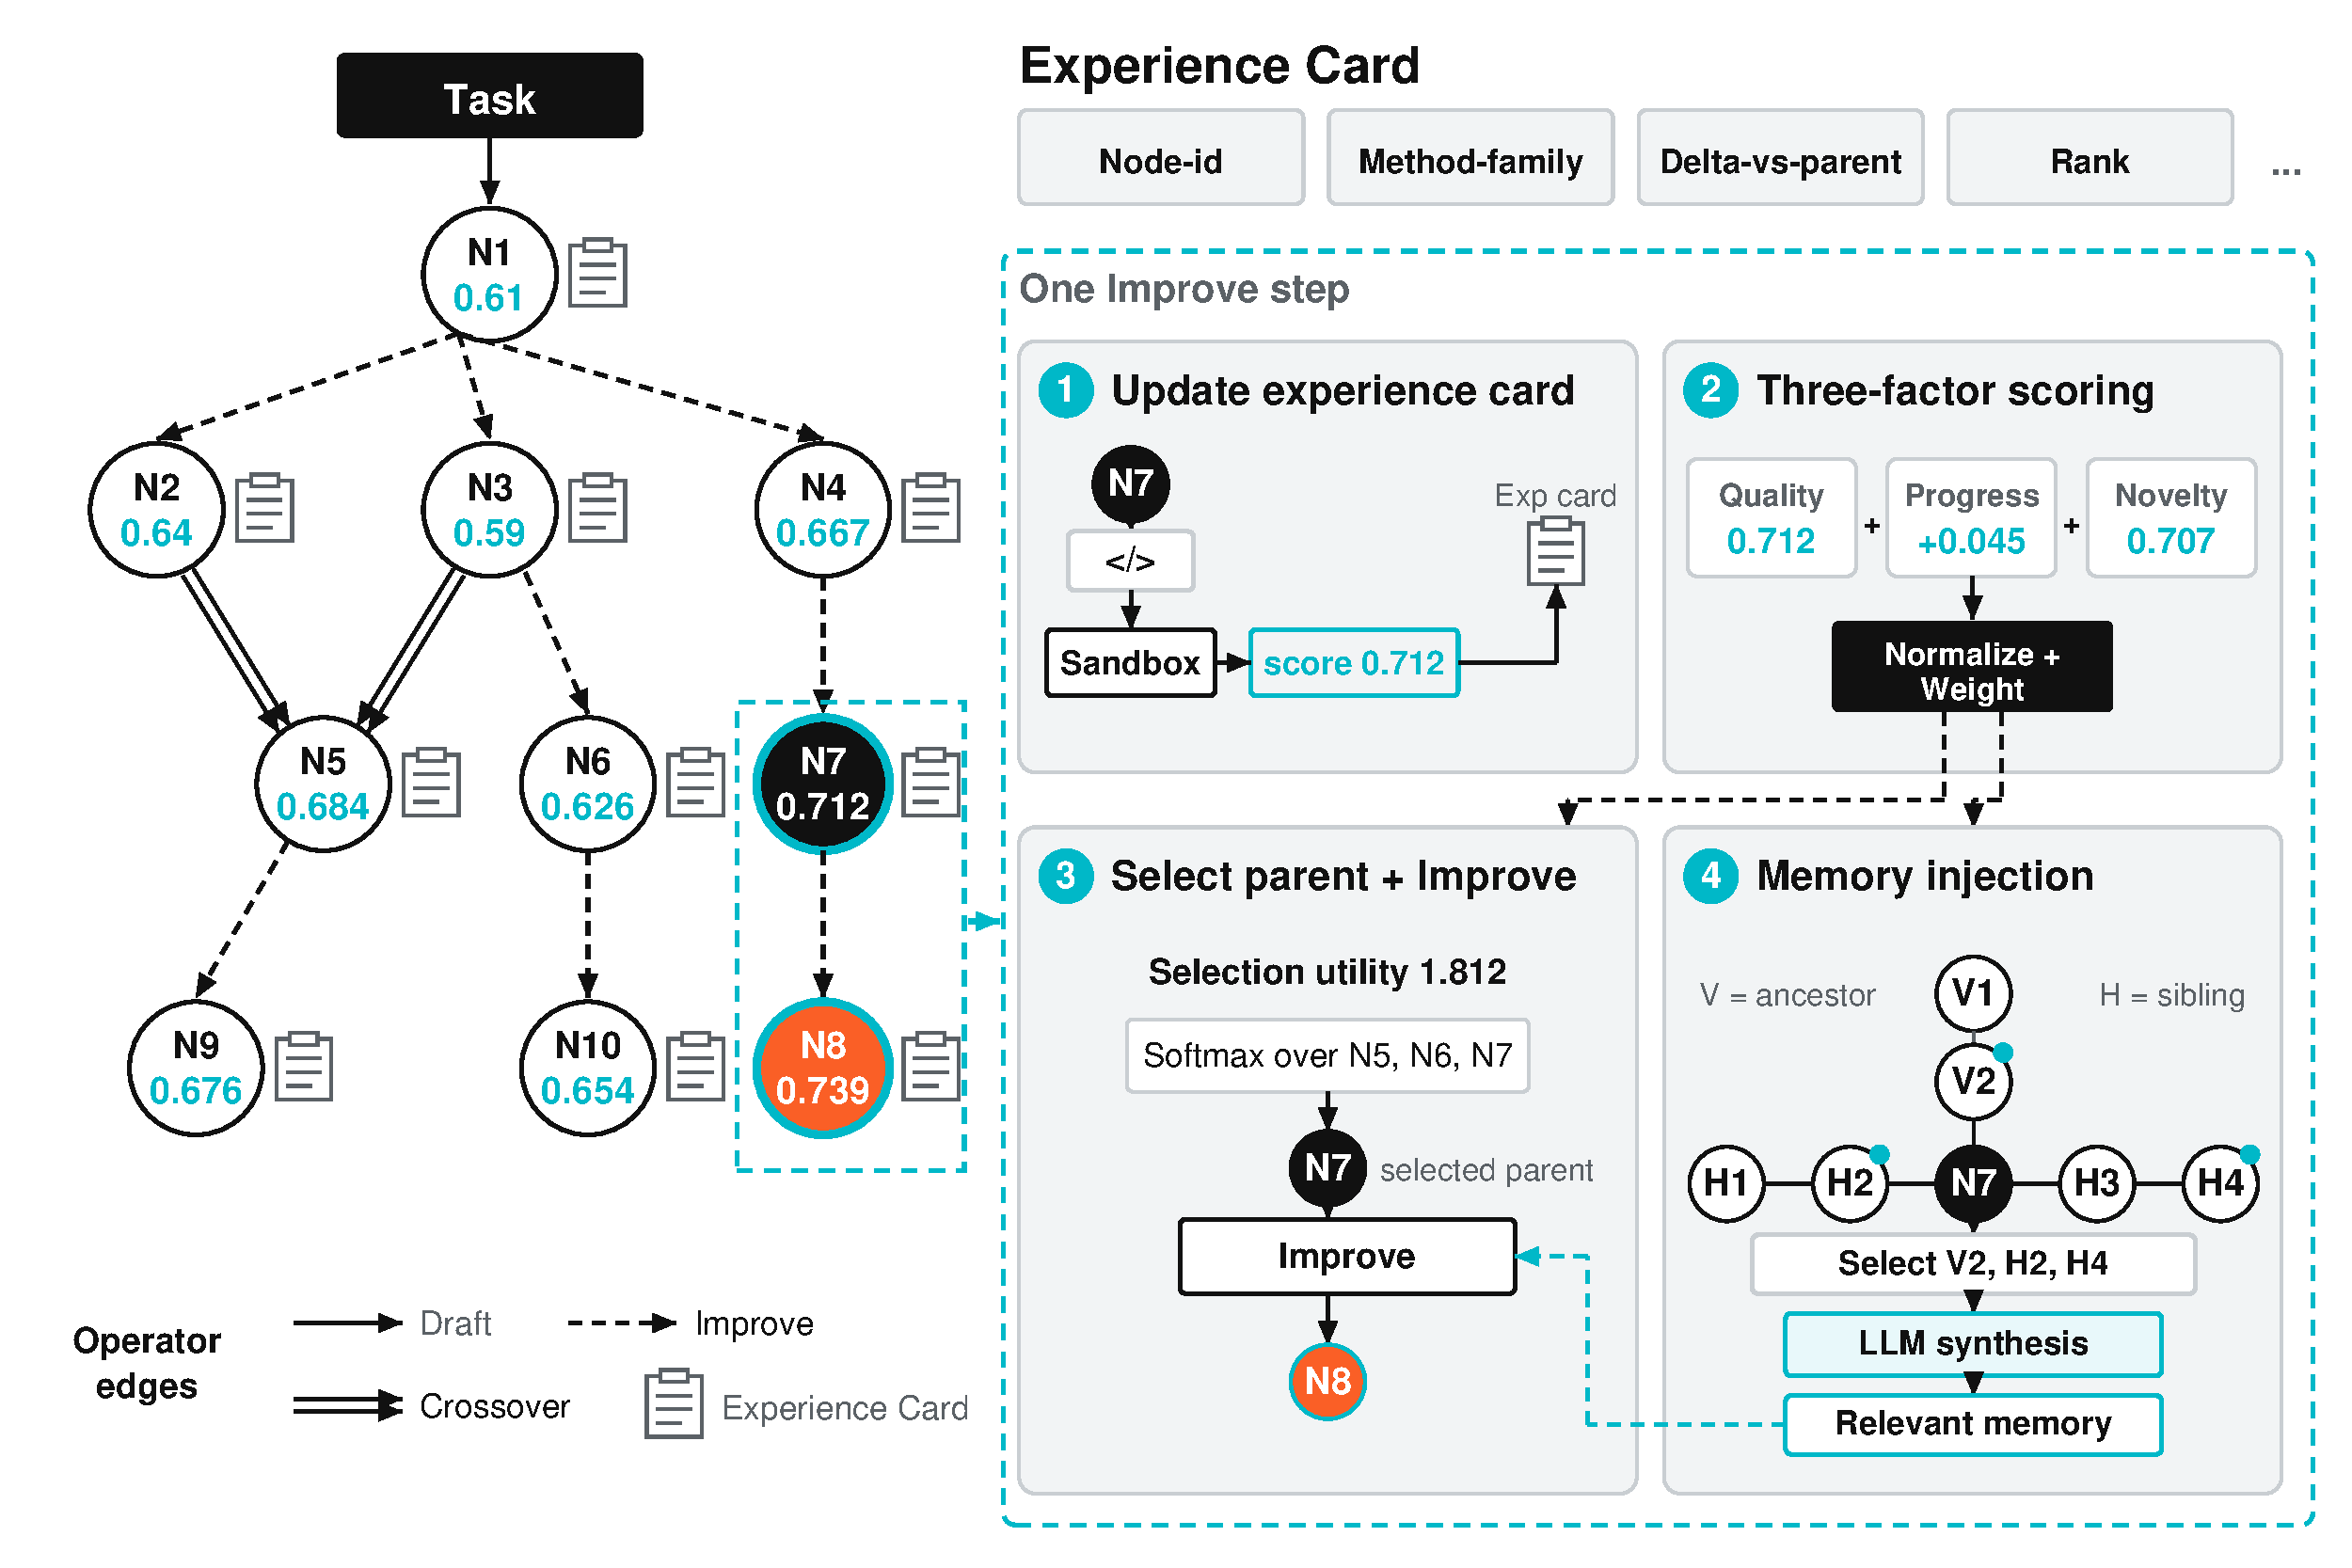
\includegraphics[width=\linewidth]{figures/experience-guided-search-final.pdf}
    \caption{\textbf{OpenMLE-Evo Search Harness.} \textbf{Left:} The search tree expands candidate solutions through drafting, improvement, and crossover operations, with each evaluated node paired with a structured experience card. \textbf{Right:} Experience-card metadata is used to update the global search state, compute parent-selection weights from quality, progress, and novelty, select the next parent, and retrieve relevant memories from key ancestors and siblings for the subsequent improvement operation.}
    \label{fig:openmle-evo-experience-guided-search}
\end{figure}

\textbf{Motivation.}
AI systems that improve AI artifacts must use execution outcomes to determine what to try next, rather than merely sample more candidates. Evolutionary test-time search operationalizes this feedback loop by maintaining executable programs, selecting parents, applying transformations, and evaluating the resulting candidates. Over long horizons, effective search therefore requires three capabilities: a persistent and queryable representation of prior attempts, compute allocation across high-quality, improving, and novel branches, and bounded context tailored to the transformation being applied.

AIDE, AIRA, and AIRA$_2$ establish iterative search over executable programs through tree- or population-based exploration, repeated execution, and candidate refinement~\citep{jiang2025aide,toledo2025airesearchagents,hambardzumyan2026aira_2}. \openmleevo{} adopts an AIRA-Evo-style population loop to compose OpenMLE's trained \textsc{Draft}, \textsc{Improve}, \textsc{Debug}, and \textsc{Crossover} operators, but redesigns how the loop uses execution evidence. Standard AIRA-Evo stores largely free-form memory, synthesizes it eagerly, selects parents primarily by scalar fitness, and supplies different operators with broadly similar histories. \openmleevo{} instead stores structured experience records, selects parents by quality, progress, and novelty, and synthesizes bounded memory on demand for the operator being invoked. The details of each component are described in the following sections, while the overall experience-guided search framework is illustrated in Figure~\ref{fig:openmle-evo-experience-guided-search}.

\subsection{Structured Experience Accumulation}
\openmleevo{} accumulates search experience at two complementary levels. First, after a candidate is evaluated in the sandbox, the harness creates a node-level \textbf{experience card}. Its core metadata is extracted deterministically from the search state and execution result, capturing the candidate’s provenance, performance, execution outcome, and resource usage. The full schema details and a grounded record are provided in Appendix~\ref{app:openmleevo-experience-records}. This gives every node a compact and consistently structured record of both the attempted change and its observed outcome. Second, the harness aggregates the cards from all evaluated nodes into a task-global experience board. The board maintains population-level statistics such as explored method families, family-wise best candidates, underexplored directions, repeated failures, score trends, and the parent graph. It therefore exposes the state of the surrounding search neighborhood, allowing a newly selected node to understand not only its own history but also how its ancestors, siblings, and related method families have performed. Together, the card and board prevent node-level signals from being lost in the expanding search space. This queryable deterministic state supplies quality, progress, and novelty to parent selection, and lineage, neighborhood, failure, and resource evidence to operation-conditioned retrieval and on-demand memory synthesis.



\subsection{Experience-Guided Parent Selection}

Original AIRA-Evo derives parent-sampling probabilities primarily from
normalized fitness. Consequently, although parent selection remains
stochastic, the search is driven almost entirely by a node's current
validation score and tends to concentrate expansion on already strong
nodes. Other informative signals, such as how much a node improves upon
its ancestry or whether it introduces a previously underexplored solution
family, are not explicitly considered.

In \openmleevo{}, we instead transform the deterministic metadata stored
in each experience card into three complementary factors: normalized
validation score $\tilde{s}_i$, normalized positive improvement over the
strongest parent $\widetilde{\Delta}_i$, and method-family novelty $\nu_i$.
For candidates $i \in \mathcal{I}$ in a sampled island, we define an
experience-guided utility and sample the next parent according to
\begin{equation}
U_i
=
\lambda_s \tilde{s}_i
+
\lambda_{\Delta} \widetilde{\Delta}_i
+
\lambda_n \nu_i,
\qquad
P(i \mid \mathcal{I})
=
\frac{\exp(U_i/\tau)}
{\sum_{j \in \mathcal{I}} \exp(U_j/\tau)}.
\label{eq:openmleevo-parent-selection}
\end{equation}

Thus, each parent-selection decision jointly considers three aspects of a
candidate: its current solution quality, the progress it achieved relative
to its lineage, and the algorithmic novelty of the direction it represents.
This produces a more comprehensive expansion policy: it preserves selection
pressure toward high-quality solutions while still allocating search budget
to candidates that demonstrate meaningful progress or introduce promising,
underexplored approaches. Detailed factor definitions and sampling procedures are provided in
Appendix~\ref{app:openmleevo-parent-selection}.

\subsection{Operation-Triggered Memory Synthesis}
The original AIRA-Evo memory path eagerly invokes a language model to summarize the history of every evaluated node by default. This spends inference budget on nodes that are never selected by a later operator, while producing a summary before the decision context that should shape it is known. \openmleevo{} separates deterministic storage from language-model synthesis: after sandbox evaluation, it preserves the experience card and experience board, but defers rich natural-language memory until an \textsc{Improve}, \textsc{Crossover}, or \textsc{Debug} call has selected its relevant nodes. It then invokes the memory model only for the selected parent(s) and their retrieved ancestors, siblings, or error-related attempts, and caches the resulting method and parent-comparison summaries. This on-demand policy avoids unnecessary calls over long search trajectories, improves the efficiency of LLM-based experience extraction, and lets an optimized operation-aware extraction template produce more relevant, higher-quality memory. Prompt templates and representative memory records are deferred to Appendix~\ref{app:openmleevo-memory-synthesis}.

\subsection{Operator-Conditioned Context Construction}
Once a parent has been sampled, \openmleevo{} constructs a small, operator-conditioned context instead of appending the full free-form history. For \textsc{Improve}, it concatenates the selected node's deterministic experience record including its validation score, improvement over its parent, method family, runtime, rank, incumbent status, and direction novelty with a vertical trace of its recent ancestors and a horizontal set of direct siblings, namely prior candidates sharing at least one parent. The sibling set is ranked by the same score--improvement--novelty utility used for parent selection, and only the most informative siblings are retained; the operator can therefore contrast the chosen trajectory with nearby alternatives rather than unrelated programs elsewhere in the search. A global experience board, recomputed from all accumulated cards, further supplies the current best method family, family-level success and failure statistics, underexplored directions, recent improvement trends, and recurring error signatures. \textsc{Crossover} applies this construction separately to both parents and adds a method-family complementarity cue, whereas \textsc{Debug} retrieves prior attempts with the same error signature, falling back to recent attempts when exact matches are unavailable. Concise method and parent-comparison summaries are generated lazily for the retrieved nodes and cached, while the core retrieval signals remain deterministic. This branch-local, bounded context avoids the redundancy of an ever-growing history and gives each operator evidence that is directly actionable for refinement, recombination, or repair. The resulting prompt also specifies the remaining search budget, remaining steps, and per-run execution limit, so that these decisions remain feasible under the task's actual computational constraints; Appendix~\ref{app:openmleevo-memory-synthesis} specifies the retrieval sets and generated fields.


